% \newcommand{\format}[2]{$#1\times10^{#2}$}
\newcommand{\format}[2]{$#1$e$#2$}


\subsection{The method of analytic solutions}

The {\it method of analytic solutions} is an extremely useful technique
for constructing exact solutions that can be used to check the accuracy
of a code.

The {\it method of analytic solutions} is used to choose $f$ and $g$
so that the exact solution to~(\ref{eq:poisson1}-\ref{eq:poisson2})
is known. For example, any sufficiently smooth 
function $w(\xv)$ will be a solution provided $f=\Delta w$
and $g = \alpha_1 {\partial w \over \partial n} + \alpha_0 w$. 
With this approach the error in the discrete solution can be easily determined. 
Two common choices for exact solutions are a low degree polynomial
% \[
%     w(\xv) = \sum c_{lmn} x^l y^m z^n ~,
% \]
or a trigonometric function such as
$w(\xv) = \cos( f_x \pi x)\cos( f_y \pi y )\cos( f_z \pi z)$. 
The trigonometric function will be used in the examples given in this section.

Table~(\ref{table:mx.sib}) shows convergence results for solutions computed
on overlapping grids for the region exterior to a sphere and interior to a larger box. The finest grid
in this case had about $6.4$ million grid points.
\begin{table}[hbt]
\begin{center}
\begin{tabular}{|l|c|c|c|c|c|} \hline\hline 
grid  & N &  $E_x$ &  $E_y$ & $E_z$ & $\grad\cdot\uv$\\ \hline 
         sib1.order4 &    40 &$8.3 e-4$ &$4.5 e-4$ &$7.5 e-4$ &$2.8 e-3$  \\ \hline
       sib1x2.order4 &    80 &$5.4 e-5$ &$2.5 e-5$ &$5.3 e-5$ &$2.1 e-4$  \\ \hline
       sib1x4.order4 &   160 &$3.4 e-6$ &$1.7 e-6$ &$3.3 e-6$ &$2.4 e-5$  \\ \hline
    rate         &     &       $3.97$ &       $4.02$ &       $3.91$ &       $3.41$  \\ \hline\hline
\end{tabular}
\caption{Sphere in a box domain, order=$4$, $t=.25$, sib, trig TZ, bc=pec, cfl=.95, ad=.1}\label{table:mx.sib}
\end{center}
\end{table}


Table~(\ref{table:mx.bis}) shows convergence results for a grid covering the interior
of a sphere.
\begin{table}[hbt]
\begin{center}
\begin{tabular}{|l|c|c|c|c|c|} \hline\hline 
grid  & N &  $E_x$ &  $E_y$ & $E_z$ & $\grad\cdot\uv$\\ \hline 
        bis1a.order4 &    10 &  $1.8\times10^{ -3}$  &  $7.2\times10^{ -4}$  &  $4.5\times10^{ -4}$  &  $6.2\times10^{ -2}$   \\ \hline
        bis2a.order4 &    20 &  $5.6\times10^{ -5}$  &  $3.0\times10^{ -5}$  &  $6.5\times10^{ -5}$  &  $5.1\times10^{ -3}$   \\ \hline
        bis3a.order4 &    40 &  $6.2\times10^{ -6}$  &  $3.4\times10^{ -6}$  &  $7.2\times10^{ -6}$  &  $3.4\times10^{ -4}$   \\ \hline
        bis4a.order4 &    80 &  $3.8\times10^{ -7}$  &  $2.6\times10^{ -7}$  &  $4.4\times10^{ -7}$  &  $2.3\times10^{ -5}$   \\ \hline
    rate            &     &       $3.99$ &       $3.75$ &       $3.32$ &       $3.80$  \\ \hline\hline
\end{tabular}
\caption{Spherical domain, nfdtd, order=$4$, $t=0.025$, bis, trig TZ, bc=pec, cfl=.8}\label{table:mx.bis}
\end{center}
\end{table}

\begin{table}[hbt]
\begin{center}
\begin{tabular}{|l|c|c|c|c|c|} \hline\hline 
grid  & N &  $E_x$ &  $E_y$ & $E_z$ & $\grad\cdot\uv$\\ \hline 
        tube1.order4 &    10 &  $8.1\times10^{ -4}$  &  $7.5\times10^{ -4}$  &  $1.3\times10^{ -3}$  &  $7.6\times10^{ -3}$   \\ \hline
        tube2.order4 &    20 &  $4.5\times10^{ -5}$  &  $5.1\times10^{ -5}$  &  $8.1\times10^{ -5}$  &  $6.9\times10^{ -4}$   \\ \hline
        tube3.order4 &    40 &  $2.6\times10^{ -6}$  &  $2.7\times10^{ -6}$  &  $3.2\times10^{ -6}$  &  $8.8\times10^{ -5}$   \\ \hline
        tube4.order4 &    80 &  $1.8\times10^{ -7}$  &  $1.8\times10^{ -7}$  &  $1.4\times10^{ -7}$  &  $3.0\times10^{ -5}$   \\ \hline
    rate            &     &       $4.04$ &       $4.04$ &       $4.43$ &       $2.69$  \\ \hline\hline
\end{tabular}
\caption{Cylinder, nfdtd, order=$4$, $t=.25$, tube, trig TZ, bc=pec, cfl=.85}\label{table:mx.tube}
\end{center}
\end{table}

\subsection{Eigenfunctions on a disk}

The eigenfunctions for a unit disk, $x^2+y^2 < 1$ are
\begin{align*}
   u_{p,n}(x,y,t) &=  {1\over \omega_{p,n}}\big\{ 
              \omega_{p,n}J_n'(\omega_{p,n} r ) sin(\theta)\cos(n \theta)
                 - {n\over r} J_n(\omega_{p,n} r ) \cos(\theta) \sin(n \theta)  \big\}   \sin(\omega_{p,n} t) \\
   v_{p,n}(x,y,t) &= -{1\over \omega_{p,n}}\big\{ 
              \omega_{p,n}J_n'(\omega_{p,n} r ) cos(\theta)\cos(n \theta) 
                 + {n\over r} J_n(\omega_{p,n} r ) \sin(\theta) \sin(n \theta)  \big\}   \sin(\omega_{p,n} t)  \\
   w_{p,n}(x,y,t) & = J_n( \omega_{p,n} r ) \cos(n \theta) \cos(\omega_{p,n} t)
                  \qquad n=0,1,2,\ldots,~p=1,2,\ldots  
\end{align*}
where for a fixed $n$, $\omega_{p,n}$ is the $p-$th zero of the derivative of the Bessel function
\[
     J_n'(\omega_{p,n})=0
\]
For $n=0$ we do not include the root $\omega_{1,n}=0$

The eigenfunctions for a circular disk define some exact solutions to the Maxwell equations.
These solutions can be used to test the accuracy of the method.
% Here are some convergence results for computing the eigenfunctions of a circular disk.
The computation is initialized with the exact values of the eigen-function for $t=0$ and $t=-\Delta t$.
The equations are integrated to time $t=1$ and the errors are computed.

The tables show results for different eigen modes.

\input \maxDoc/nfdtd.sic.order4.eigenMode000.table.tex

\input \maxDoc/nfdtd.sic.order4.eigenMode120.table.tex

\input \maxDoc/nfdtd.sic.order4.eigenMode430.table.tex

\renewcommand{\figWidth}{.45\linewidth}
\begin{figure}
\begin{center}
\includegraphics[width=\figWidth]{figures/diskEigenMode43Hz}
\includegraphics[width=\figWidth]{figures/diskEigenMode43Ex}
% \epsfig{file=\maxDoc/diskEigenMode43Hz.ps,width=\figWidth}  
% \epsfig{file=\maxDoc/diskEigenMode43Ex.ps,width=\figWidth}  
\end{center}
\caption{Eigenmode $(4,3)$ of the circular disk.}
\end{figure}

\subsection{Eigenfunctions of a cylinder}

Consider a cylinder of length $d$, denoted by $C(d)$.
The eigenfunctions of the domain $C(d)$ are
\begin{align*}
  u_{p,n,k}(r,\theta,z,t) &= - { (k\pi/d) \over \lambda^2 }
       \big\{ 
           \lambda J_n'(\lambda r ) cos(\theta)\cos(n \theta) 
                        + {n\over r} J_n(\lambda r ) \sin(\theta) \sin(n \theta)  \big\} 
               \sin(k \pi z/d)  \cos(\omega t)  \\
  v_{p,n,k}(r,\theta,z,t) &=   -{ (k\pi/d) \over \lambda^2} 
      \big\{ \lambda J_n'(\lambda r) sin(\theta)\cos(n \theta)
                 - {n\over r} J_n(\lambda r ) \cos(\theta) \sin(n \theta)  \big\}  
                          \sin(k \pi z/d)  \cos(\omega t) \\
  w_{p,n,k}(r,\theta,z,t) & = J_n( \lambda r ) \cos(n \theta) \cos(k \pi z/d) \cos(\omega t) \\
       \lambda &= \lambda_{p,n}, \qquad \mbox{with $J_n(\lambda_{p,n})=0$,} \\
       \omega &= \omega_{p,n,k} = \sqrt{(k\pi/d)^2 + \lambda_{p,n}^2} \\
        n=0,1,2,3,\ldots,&\quad p=1,2,3,\ldots,\quad k=1,2,3,\ldots
\end{align*}

Tables~(\ref{table:mx.tube001}-\ref{table:mx.tube112}) presents some convergence results.

% nfdtd.tube.order4.eigenMode001.table.tex
\begin{table}[hbt]
\begin{center}
\begin{tabular}{|l|c|c|c|c|c|} \hline\hline 
grid  & N &  $E_x$ &  $E_y$ & $E_z$ & $\grad\cdot\uv$\\ \hline 
        tube1.order4 &    10 &  $2.2\times10^{ -5}$  &  $2.2\times10^{ -5}$  &  $1.5\times10^{ -5}$  &  $6.7\times10^{ -4}$   \\ \hline
        tube2.order4 &    20 &  $1.1\times10^{ -6}$  &  $1.1\times10^{ -6}$  &  $1.1\times10^{ -6}$  &  $3.8\times10^{ -5}$   \\ \hline
        tube3.order4 &    40 &  $1.1\times10^{ -7}$  &  $1.1\times10^{ -7}$  &  $7.0\times10^{ -8}$  &  $1.3\times10^{ -6}$   \\ \hline
    rate            &     &       $3.83$ &       $3.82$ &       $3.85$ &       $4.51$  \\ \hline\hline
\end{tabular}
\caption{nfdtd, order=$4$, $t=0.1$, tube, eigen-mode 0,0,1, cfl=0.75}\label{table:mx.tube001}
\end{center}
\end{table}

% nfdtd.tube.order4.eigenMode112.table.tex
% \begin{table}[hbt]
% \begin{center}
% \begin{tabular}{|l|c|c|c|c|c|} \hline\hline 
% grid  & N &  $E_x$ &  $E_y$ & $E_z$ & $\grad\cdot\uv$\\ \hline 
%         tube1.order4 &    10 &  $1.1\times10^{ -3}$  &  $5.6\times10^{ -4}$  &  $1.2\times10^{ -3}$  &  $5.7\times10^{ -3}$   \\ \hline
%         tube2.order4 &    20 &  $7.1\times10^{ -5}$  &  $3.1\times10^{ -5}$  &  $9.1\times10^{ -5}$  &  $3.8\times10^{ -4}$   \\ \hline
%         tube3.order4 &    40 &  $5.5\times10^{ -6}$  &  $2.8\times10^{ -6}$  &  $5.9\times10^{ -6}$  &  $4.2\times10^{ -5}$   \\ \hline
%         tube4.order4 &    80 &  $3.5\times10^{ -7}$  &  $1.7\times10^{ -7}$  &  $3.8\times10^{ -7}$  &  $2.5\times10^{ -6}$   \\ \hline
%     rate            &     &       $3.86$ &       $3.84$ &       $3.88$ &       $3.67$  \\ \hline\hline
% \end{tabular}
% \caption{nfdtd, order=$4$, $t=0.1$, tube, eigen-mode 1,1,2, cfl=.5}\label{table:mx.tube}
% \end{center}
% \end{table}

% nfdtd.tube.order4.eigenMode112.table.tex
\begin{table}[hbt]
\begin{center}
\begin{tabular}{|l|c|c|c|c|c|} \hline\hline 
grid  & N &  $E_x$ &  $E_y$ & $E_z$ & $\grad\cdot\uv$\\ \hline 
        tube1.order4 &    10 &  $7.6\times10^{ -3}$  &  $3.4\times10^{ -3}$  &  $9.9\times10^{ -3}$  &  $6.5\times10^{ -3}$   \\ \hline
        tube2.order4 &    20 &  $5.7\times10^{ -4}$  &  $2.5\times10^{ -4}$  &  $7.3\times10^{ -4}$  &  $1.5\times10^{ -3}$   \\ \hline
        tube3.order4 &    40 &  $3.7\times10^{ -5}$  &  $1.6\times10^{ -5}$  &  $4.7\times10^{ -5}$  &  $3.3\times10^{ -5}$   \\ \hline
        tube4.order4 &    80 &  $2.3\times10^{ -6}$  &  $1.0\times10^{ -6}$  &  $3.0\times10^{ -6}$  &  $3.0\times10^{ -6}$   \\ \hline
    rate            &     &       $3.90$ &       $3.90$ &       $3.90$ &       $3.87$  \\ \hline\hline
\end{tabular}
\caption{nfdtd, order=$4$, $t=.25$, tube, eigen-mode 1,1,2, cfl=.9}\label{table:mx.tube}
\end{center}
\end{table}

\begin{table}[hbt]
\begin{center}
\begin{tabular}{|l|c|c|c|c|c|} \hline\hline 
grid  & N &  $E_x$ &  $E_y$ & $E_z$ & $\grad\cdot\uv$\\ \hline 
       tube1a.order4 &    10 &$1.4 e-3$ &$1.2 e-3$ &$5.2 e-3$ &$3.8 e-2$  \\ \hline
       tube2a.order4 &    20 &$1.1 e-4$ &$2.9 e-5$ &$3.4 e-4$ &$3.4 e-3$  \\ \hline
       tube3a.order4 &    40 &$5.0 e-6$ &$2.4 e-6$ &$1.2 e-5$ &$7.0 e-5$  \\ \hline
       tube4a.order4 &    80 &$2.7 e-7$ &$1.8 e-7$ &$4.6 e-7$ &$6.2 e-6$  \\ \hline
    rate            &     &       $4.16$ &       $4.17$ &       $4.53$ &       $4.34$  \\ \hline\hline
\end{tabular}
\caption{Maximum errors in computing 
         eigen-mode $(1,1,2)$ of a cylinder, order=$4$, $t=1.0$, tube,  cfl=.9, ad=.5(?)}\label{table:mx.tube}
\end{center}
\end{table}

\begin{table}[hbt]
\begin{center}
\begin{tabular}{|l|c|c|c|c|c|} \hline\hline 
grid  & N &  $E_x$ &  $E_y$ & $E_z$ & $\grad\cdot\uv$\\ \hline 
       tube1a.order4 &    10 &$1.8 e-3$ &$8.9 e-4$ &$1.8 e-3$ &$3.0 e-2$  \\ \hline
       tube2a.order4 &    20 &$6.7 e-5$ &$2.7 e-5$ &$8.0 e-5$ &$1.2 e-3$  \\ \hline
       tube3a.order4 &    40 &$2.8 e-6$ &$1.4 e-6$ &$5.3 e-6$ &$8.8 e-5$  \\ \hline
       tube4a.order4 &    80 &$1.9 e-7$ &$9.1 e-8$ &$3.1 e-7$ &$7.7 e-6$  \\ \hline
    rate            &     &       $4.43$ &       $4.40$ &       $4.13$ &       $3.96$  \\ \hline\hline
\end{tabular}
\caption{nfdtd, order=$4$, $t=1.0$, tube, eigen-mode 1,1,2, cfl=.95, ad=.1}\label{table:mx.tube}
\end{center}
\end{table}


\begin{table}[hbt]
\begin{center}
\begin{tabular}{|l|c|c|c|c|c|} \hline\hline 
grid  & N &  $E_x$ &  $E_y$ & $E_z$ & $\grad\cdot\uv$\\ \hline 
       tube1a.order4 &    10 &$3.8 e-2$ &$3.8 e-2$ &$1.8 e-1$ &$1.2 e-1$  \\ \hline
       tube2a.order4 &    20 &$2.5 e-3$ &$2.5 e-3$ &$1.4 e-2$ &$3.6 e-3$  \\ \hline
       tube3a.order4 &    40 &$2.0 e-4$ &$2.0 e-4$ &$9.5 e-4$ &$4.9 e-4$  \\ \hline
       tube4a.order4 &    80 &$1.4 e-5$ &$1.4 e-5$ &$6.2 e-5$ &$3.6 e-5$  \\ \hline
    rate            &     &       $3.79$ &       $3.79$ &       $3.85$ &       $3.80$  \\ \hline\hline
\end{tabular}
\caption{Maximum errors in computing eigen-mode $(2,3,3)$,
          nfdtd, order=$4$, $t=1.0$, tube,  cfl=.95, ad=.25 }\label{table:mx.tube}
\end{center}
\end{table}

\begin{table}[hbt]
\begin{center}
\begin{tabular}{|l|c|c|c|c|c|} \hline\hline 
grid  & N &  $E_x$ &  $E_y$ & $E_z$ & $\grad\cdot\uv$\\ \hline 
       tube1a.order4 &    10 &$2.5 e-2$ &$2.5 e-2$ &$1.2 e-1$ &$1.1 e-1$  \\ \hline
       tube2a.order4 &    20 &$1.4 e-3$ &$1.4 e-3$ &$7.5 e-3$ &$4.2 e-3$  \\ \hline
       tube3a.order4 &    40 &$1.1 e-4$ &$1.1 e-4$ &$5.1 e-4$ &$4.9 e-4$  \\ \hline
       tube4a.order4 &    80 &$7.4 e-6$ &$7.4 e-6$ &$3.3 e-5$ &$3.5 e-5$  \\ \hline
    rate            &     &       $3.89$ &       $3.89$ &       $3.94$ &       $3.78$  \\ \hline\hline
\end{tabular}
\caption{nfdtd, order=$4$, $t=1.0$, tube, eigen-mode 2,3,3, cfl=.95, ad=.125}\label{table:mx.tube}
\end{center}
\end{table}

\renewcommand{\figWidth}{.45\linewidth}
\begin{figure}
\begin{center}
\includegraphics[width=\figWidth]{figures/cylEigen-tube3-4-mode233-Ex}
\includegraphics[width=\figWidth]{figures/cylEigen-tube3-4-mode233-Ez}
%\epsfig{file=\maxDoc/cylEigen-tube3-4-mode233-Ex.ps,width=\figWidth}  
% \epsfig{file=\maxDoc/cylEigen-tube3-4-mode233-Ez.ps,width=\figWidth}  
\end{center}
\caption{Eigenmode $(2,3,3)$ of a cylinder, grid=tube3.order4.}
\end{figure}


\subsection{Scattering by a cylinder}

The scattering of a plane wave by a two-dimensional cylinder or radius $a$ is considered.
For an incident field 
\[
     \Ev^i = -\hat{y} Z e^{-ikx}, \qquad   H_z^i = \hat{z} e^{-ikx}, \quad Z=\sqrt{\mu/\eps},
\] 
the scattered field is given by
\begin{align*}
  H_z^s &= - \sum_{n=0}^\infty \epsilon_n (-i)^n { J_n'(ka) \over H_n^{(1)'}(ka)} H_n^{(1)}(k\rho) \cos( n \phi )
\end{align*}
where $J_n$ and $Y_n$ are the Bessel functions and $H_n^{(1)}(z)= J_n + i Y_n $ is the Hankel function
of the first kind and $\epsilon_0=1$, $\epsilon_n=2$, $n=1,2,\ldots$.

In real space the solution will be given by $H_z^s(\xv,t) = Re(H_z^s(\xv,\omega) e^{-i\omega t})$. **check**



The solution is computed on a large domain and the error is computed within the region $r<2$.

% cibcb: [-10,10] background
% >>> Maxwell NFDTD: t=5.00e+00, dt=9.6e-03 orderX=4 orderT=4 ad=0.10(order=4) |div(E)|=4.44e-03, (520 steps)
% -->t=1.3000e+01 dt=9.6e-03 Errors:[3.6048e-04,4.7703e-04,7.2694e-05,], max(u):[7.9299e-01,9.9473e-01,1.0549e+00,]
% -->t=1.4000e+01 dt=9.6e-03 Errors:[3.5698e-04,4.8309e-04,7.0580e-05,], max(u):[7.9299e-01,9.9473e-01,1.0549e+00,]
% -->t=1.5000e+01 dt=9.6e-03 Errors:[3.5448e-04,4.8196e-04,6.8664e-05,], max(u):[7.9299e-01,9.9473e-01,1.0549e+00,]
% -->t=1.6000e+01 dt=9.6e-03 Errors:[3.5420e-04,4.8256e-04,6.7707e-05,], max(u):[7.9299e-01,9.9473e-01,1.0549e+00,]
% -->t=1.7000e+01 dt=9.6e-03 Errors:[3.5436e-04,4.8524e-04,6.7498e-05,], max(u):[7.9299e-01,9.9472e-01,1.0549e+00,]
% ***
% -->t=1.8000e+01 dt=9.6e-03 Errors:[3.5342e-04,4.8827e-04,4.5487e-04,], max(u):[7.9300e-01,9.9473e-01,1.0549e+00,]
% -->t=1.9000e+01 dt=9.6e-03 Errors:[4.2799e-04,1.0404e-03,1.1630e-03,], max(u):[7.9300e-01,9.9470e-01,1.0548e+00,]

% ===== cibc2b: [-15,15] background EM2: (cibc2b.out)
% -->t=2.4000e+01 dt=4.8e-03 Errors:[2.4908e-05,3.1177e-05,5.0199e-06,], max(u):[7.9310e-01,9.9490e-01,1.0548e+00,]
% -->t=2.5000e+01 dt=4.8e-03 Errors:[2.4695e-05,3.1619e-05,4.8912e-06,], max(u):[7.9311e-01,9.9490e-01,1.0548e+00,]
% -->t=2.6000e+01 dt=4.8e-03 Errors:[2.4570e-05,3.1923e-05,4.7896e-06,], max(u):[7.9311e-01,9.9490e-01,1.0548e+00,]
% -->t=2.7000e+01 dt=4.8e-03 Errors:[2.4547e-05,3.2046e-05,4.6754e-06,], max(u):[7.9311e-01,9.9490e-01,1.0548e+00,]
% *****
% -->t=2.8000e+01 dt=4.8e-03 Errors:[2.4360e-05,8.5957e-05,9.6160e-05,], max(u):[7.9311e-01,9.9490e-01,1.0548e+00,]
% -->t=2.9000e+01 dt=4.8e-03 Errors:[7.0764e-05,1.8848e-04,2.3625e-04,], max(u):[7.9311e-01,9.9489e-01,1.0548e+00,]
% -->t=3.0000e+01 dt=4.8e-03 Errors:[1.8402e-04,3.2407e-04,2.6661e-04,], max(u):[7.9315e-01,9.9508e-01,1.0548e+00,]

\begin{table}[hbt]
\begin{center}
\begin{tabular}{|l|c|c|c|c|c|} \hline\hline 
grid  & $h_0/h$ &  $E_x$ &  $E_y$ & $H_z$ & $\grad\cdot\uv$\\ \hline 
cibc.order4  & 1 &  $3.5436e-04$  & $4.8524e-04$ & $6.7498e-05$ & $4.44e-03$   \\ \hline
cibc2.order4 & 2 &  $2.4547e-05$  & $3.2046e-05$ & $4.6754e-06$ & $3.58e-04$   \\ \hline
\end{tabular}
\caption{Errors in the scattering of a plane wave by a cylinder, order=$4$, **check div(E) values}\label{table:scatCyl}
\end{center}
\end{table}

% **** cic3.order4  kx=1
% -->t=3.0000e+00 dt=3.7e-03 Errors:[1.7550e-06,2.6365e-06,5.2371e-07,], max(u):[7.93e-01,1.06e+00,1.16e+00,]
% >>> Maxwell NFDTD: t=3.00e+00, dt=3.7e-03 TS=ME orderX=4 orderT=4 ad=0.10(order=4) |div(E)|=2.92e-05, |div(E)|/|grad(E)|=1.72e-07 (804 steps)
% **** cic2.order4  kx=1
% -->t=3.0000e+00 dt=7.5e-03 Errors:[2.6977e-05,4.0047e-05,8.3604e-06,], max(u):[7.93e-01,1.06e+00,1.16e+00,]
% >>> Maxwell NFDTD: t=3.00e+00, dt=7.5e-03 TS=ME orderX=4 orderT=4 ad=0.10(order=4) |div(E)|=4.08e-04, |div(E)|/|grad(E)|=4.75e-06 (402 steps)
% ***** cic.order4  kx=1
% -->t=3.0000e+00 dt=1.5e-02 Errors:[3.9987e-04,5.8890e-04,1.2981e-04,], max(u):[7.93e-01,1.06e+00,1.16e+00,]
% >>> Maxwell NFDTD: t=3.00e+00, dt=1.5e-02 TS=ME orderX=4 orderT=4 ad=0.10(order=4) |div(E)|=5.08e-03, |div(E)|/|grad(E)|=4.52e-04 (201 steps)

% \begin{table}[hbt]
% \begin{center}
% \begin{tabular}{|l|c|c|c|c|c|} \hline\hline 
% grid  & $h_0/h$ &  $E_x$ &  $E_y$ & $H_z$ & $\|\grad\cdot\uv\|/\|\grad\uv\|$\\ \hline 
% cic.order4  & 1 &  $4.00-04$  & $5.89e-4$ & $1.30e-4$ & $4.52e-04$   \\ \hline
% cic2.order4 & 2 &  $2.70e-5$  & $4.00e-5$ & $8.36e-6$ & $4.75e-06$   \\ \hline
% cic3.order4 & 4 &  $1.76e-6$  & $2.64e-6$ & $5.24e-7$ & $1.72e-07$   \\ \hline
% \end{tabular}
% \caption{Errors in the scattering of a plane wave by a cylinder, order=$4$, $t=3.$, **check gradE}\label{table:scatCyl2}
% \end{center}
% \end{table}

% These are from maxwell/conv/results/nfdtd.scattering.cic.order4.table.tex
\begin{table}[hbt]
\begin{center}
\begin{tabular}{|l|c|c|c|c|c|} \hline\hline 
grid  & N &  $E_x$ &  $E_y$ & $H_z$ & $\|\grad\cdot\Ev\|/\|\grad\Ev\|$\\ \hline 
cic.order4 &   121 &  $4.1e{ -4}$  &  $6.0e{ -4}$  &  $1.3e{ -4}$  &  $8.6e{ -4}$   \\ \hline
cic2.order4 &   241 &  $2.8e{ -5}$  &  $4.1e{ -5}$  &  $8.3e{ -6}$  &  $7.0e{ -5}$   \\ \hline
cic3.order4 &   481 &  $1.8e{ -6}$  &  $2.7e{ -6}$  &  $5.2e{ -7}$  &  $5.0e{ -6}$   \\ \hline
    rate            &     &       $3.93$ &       $3.92$ &       $4.00$ &       $3.74$  \\ \hline\hline
\end{tabular}
\caption{Errors in the scattering of a plane wave by a cylinder, order=$4$, $t=3.$, cic, scattering, cfl=.95, (exact solution used as far field BC)}\label{table:mx.cic}
\end{center}
\end{table}


\renewcommand{\figWidth}{.32\linewidth}
\begin{figure}
\begin{center}
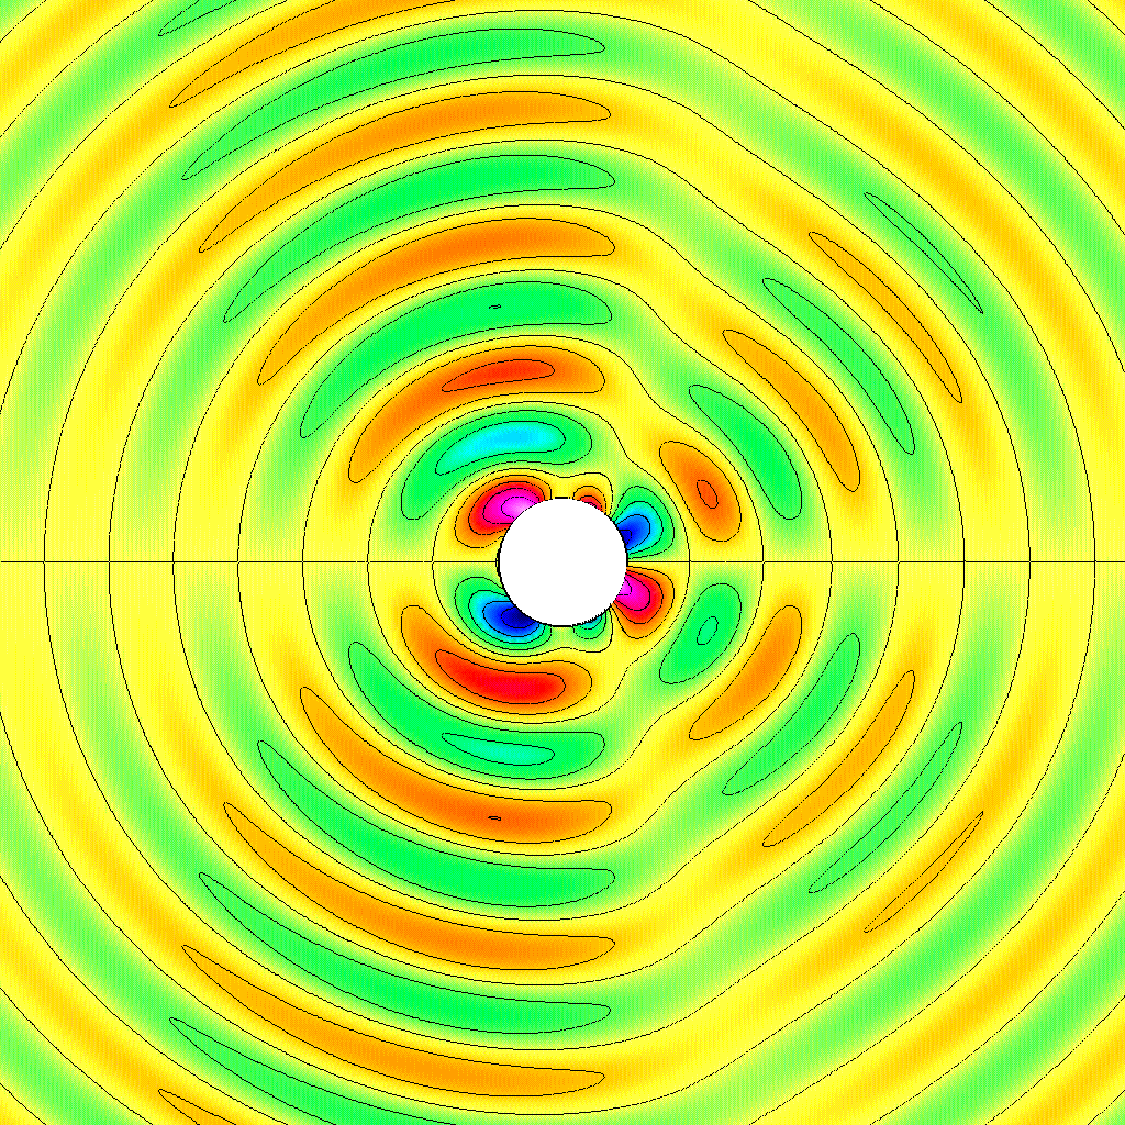
\includegraphics[width=\figWidth]{figures/scatCyl-cibc2a-order4Ex}
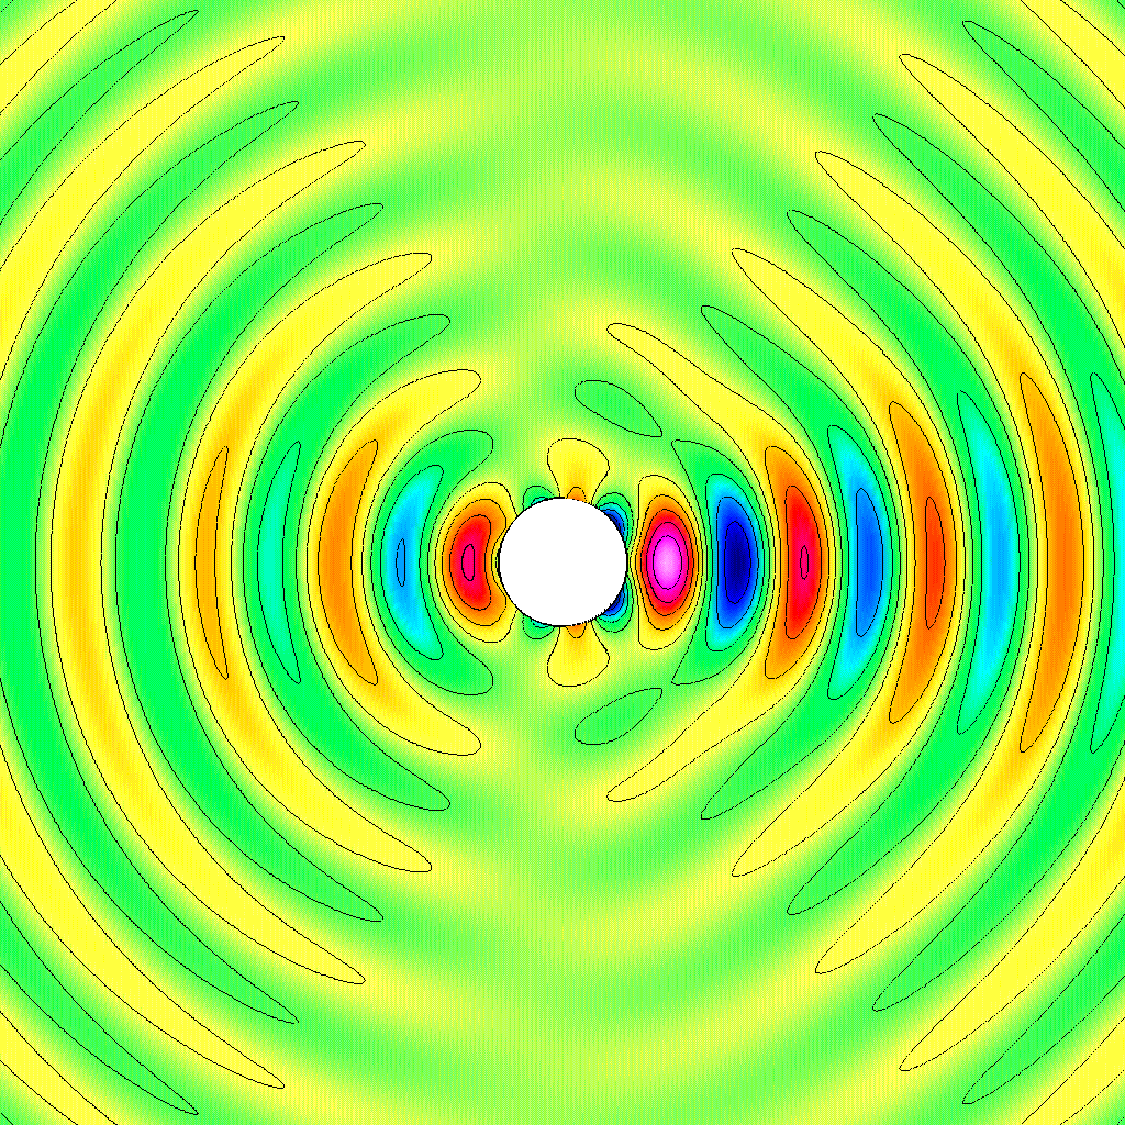
\includegraphics[width=\figWidth]{figures/scatCyl-cibc2a-order4Ey}
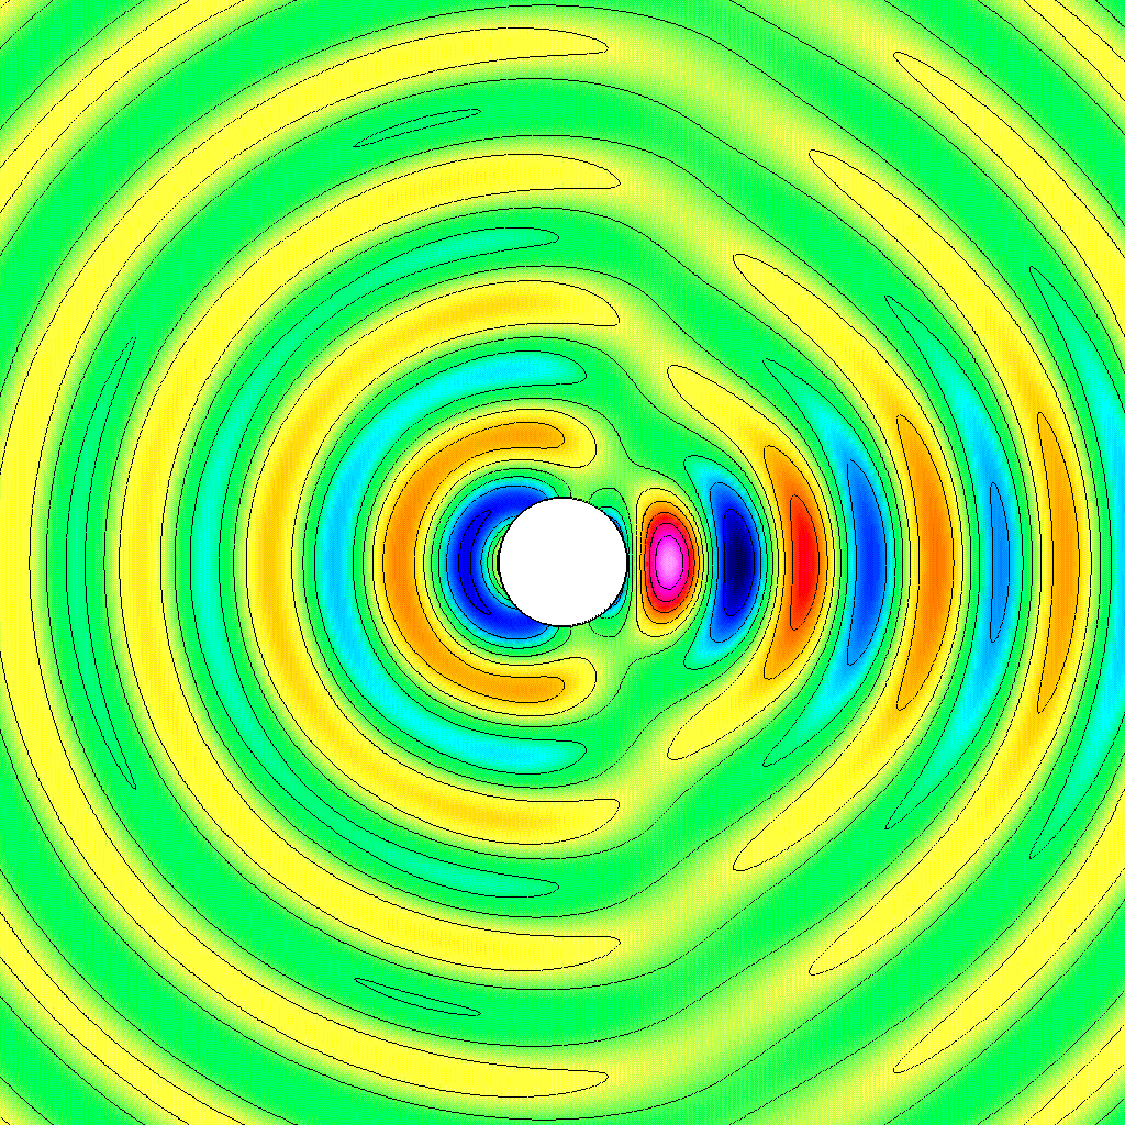
\includegraphics[width=\figWidth]{figures/scatCyl-cibc2a-order4Hz}
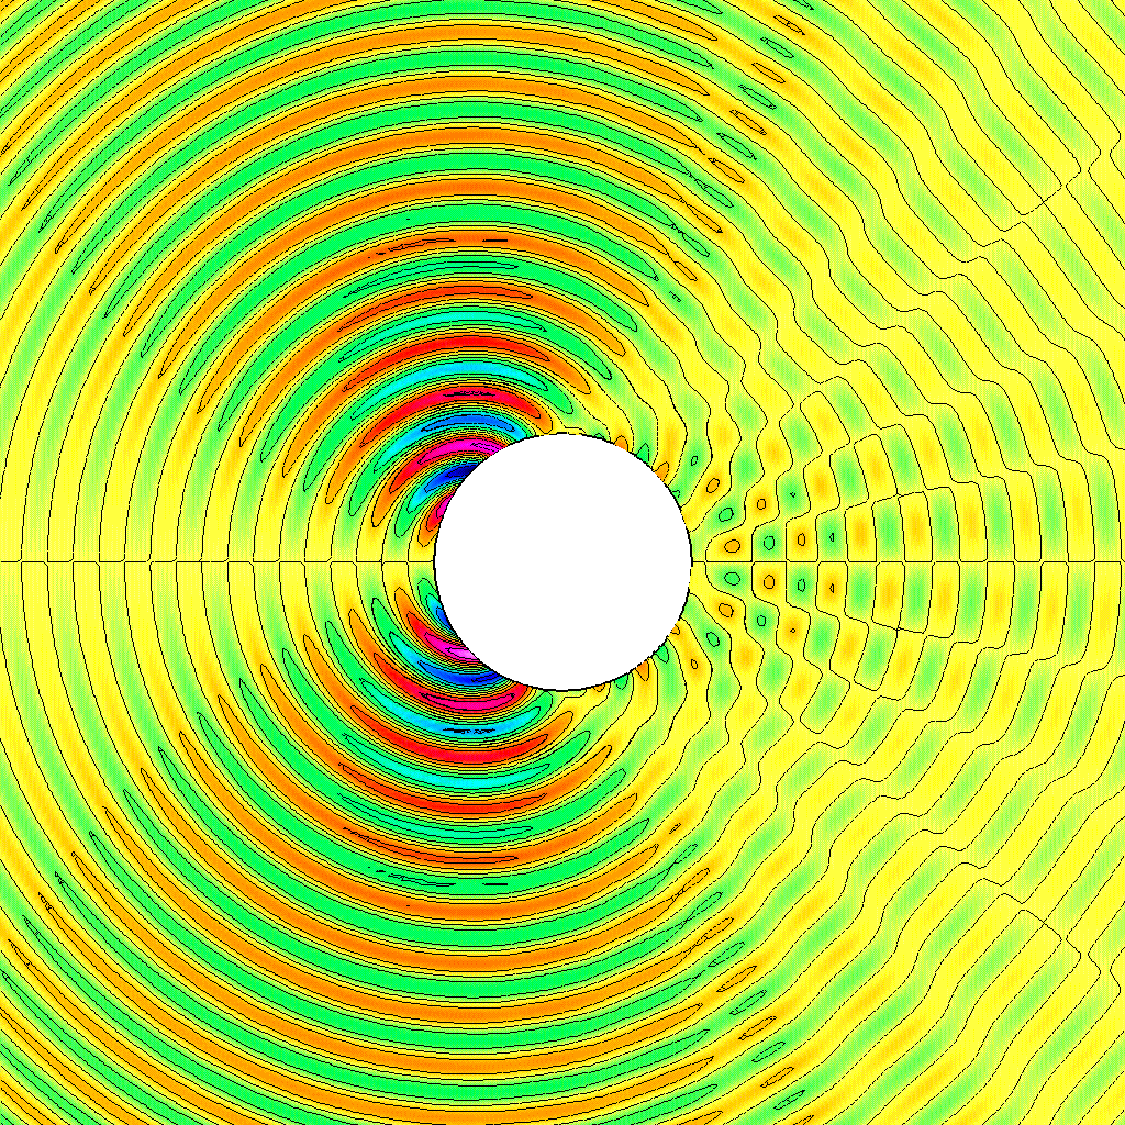
\includegraphics[width=\figWidth]{figures/scatCyl-cibc2a-order4-k5-Ex}
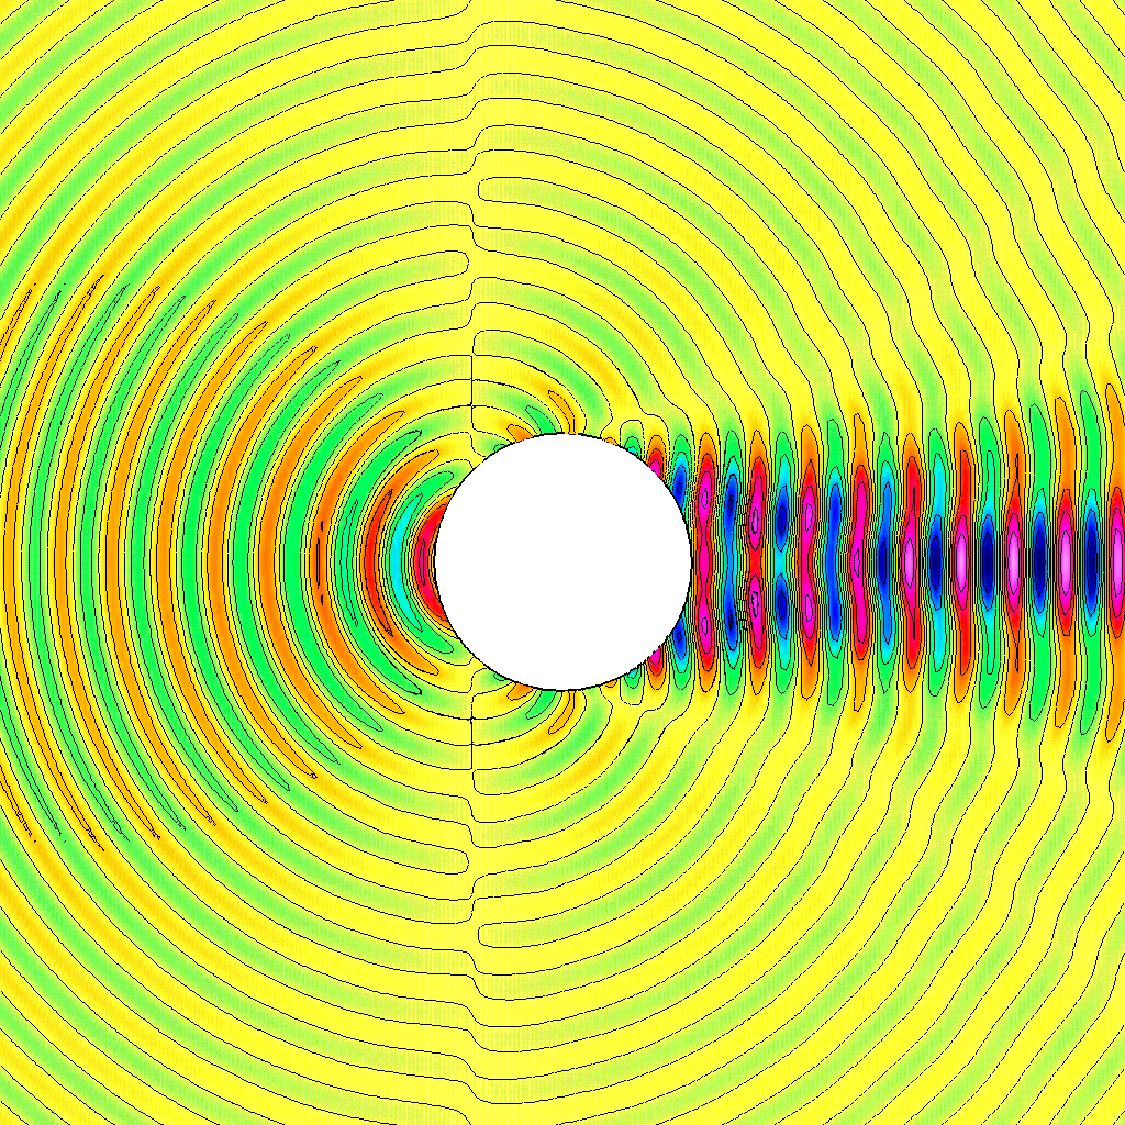
\includegraphics[width=\figWidth]{figures/scatCyl-cibc2a-order4-k5-Ey}
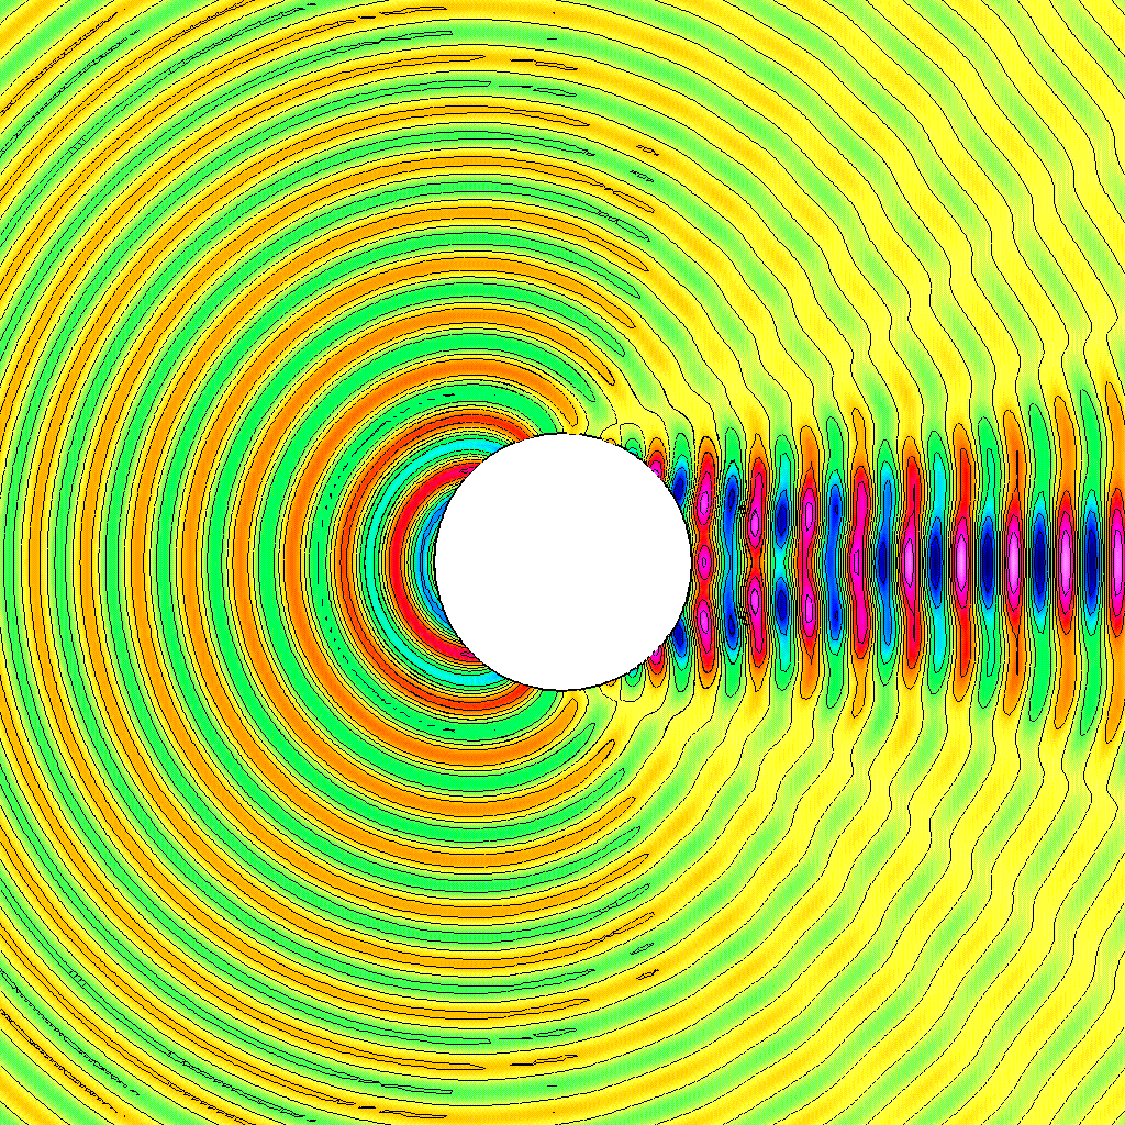
\includegraphics[width=\figWidth]{figures/scatCyl-cibc2a-order4-k5-Hz}
% 
%- \epsfig{file=\maxDoc/scatCyl.cibc2a.order4Ex.ps,width=\figWidth}  
%- \epsfig{file=\maxDoc/scatCyl.cibc2a.order4Ey.ps,width=\figWidth}  
%- \epsfig{file=\maxDoc/scatCyl.cibc2a.order4Hz.ps,width=\figWidth}  
%- \epsfig{file=\maxDoc/scatCyl.cibc2a.order4.k5.Ex.ps,width=\figWidth}  
%- \epsfig{file=\maxDoc/scatCyl.cibc2a.order4.k5.Ey.ps,width=\figWidth}  
%- \epsfig{file=\maxDoc/scatCyl.cibc2a.order4.k5.Hz.ps,width=\figWidth}  
\end{center}
\caption{Scattering of a plane wave by a cylinder. Top: scattered field $E_x$, $E_y$ and $H_z$ for $k a = 1/2$.
           Bottom: scattered field $E_x$, $E_y$ and $H_z$ for $k a = 5/2$}
\end{figure}

\begin{figure}
\begin{center}
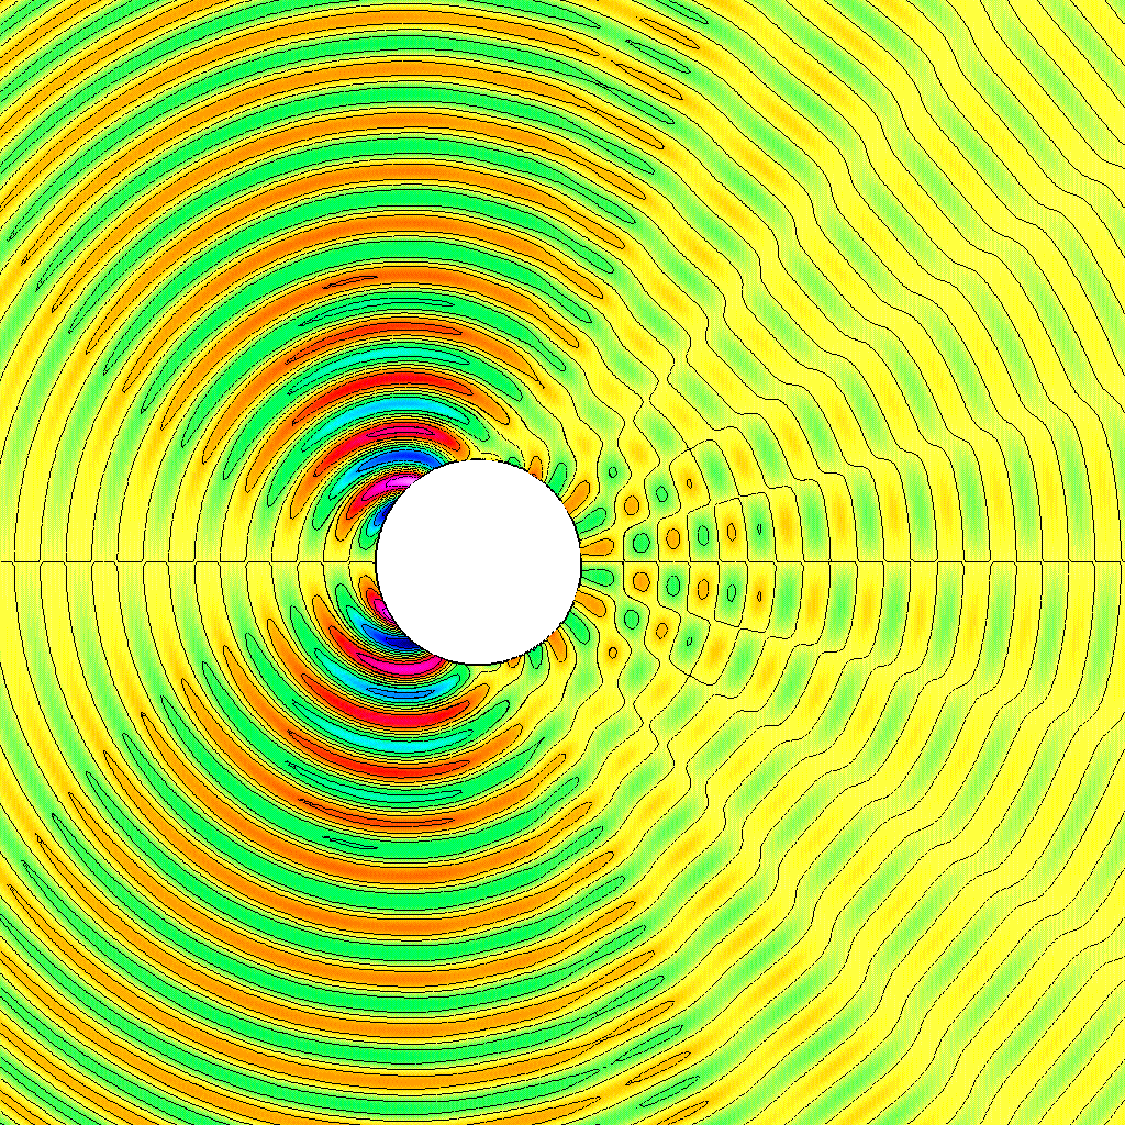
\includegraphics[width=\figWidth]{figures/scatCyl-cibc2-order4-k4-ExTotal}
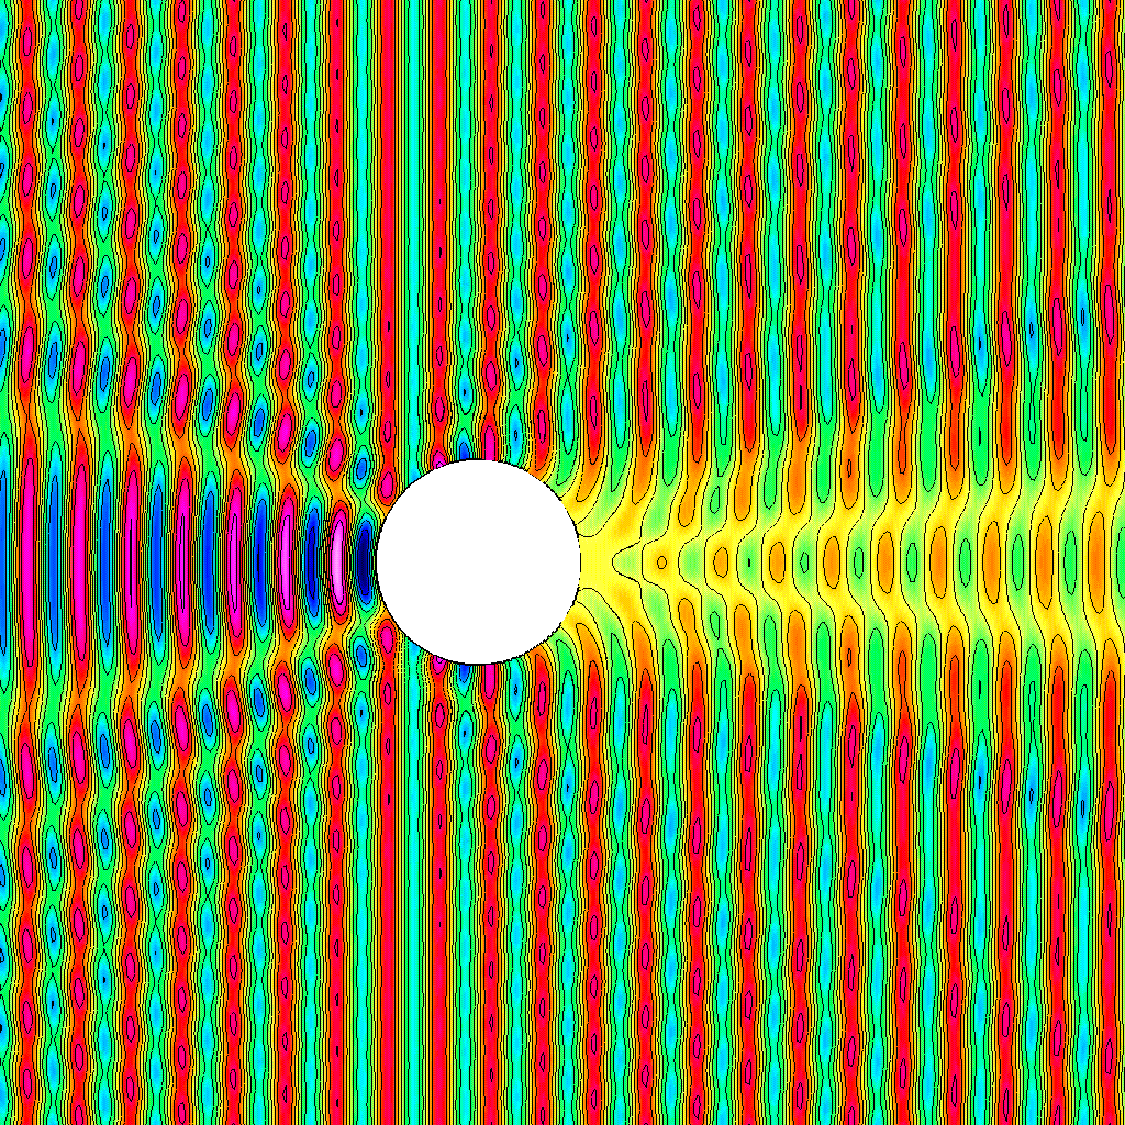
\includegraphics[width=\figWidth]{figures/scatCyl-cibc2-order4-k4-EyTotal}
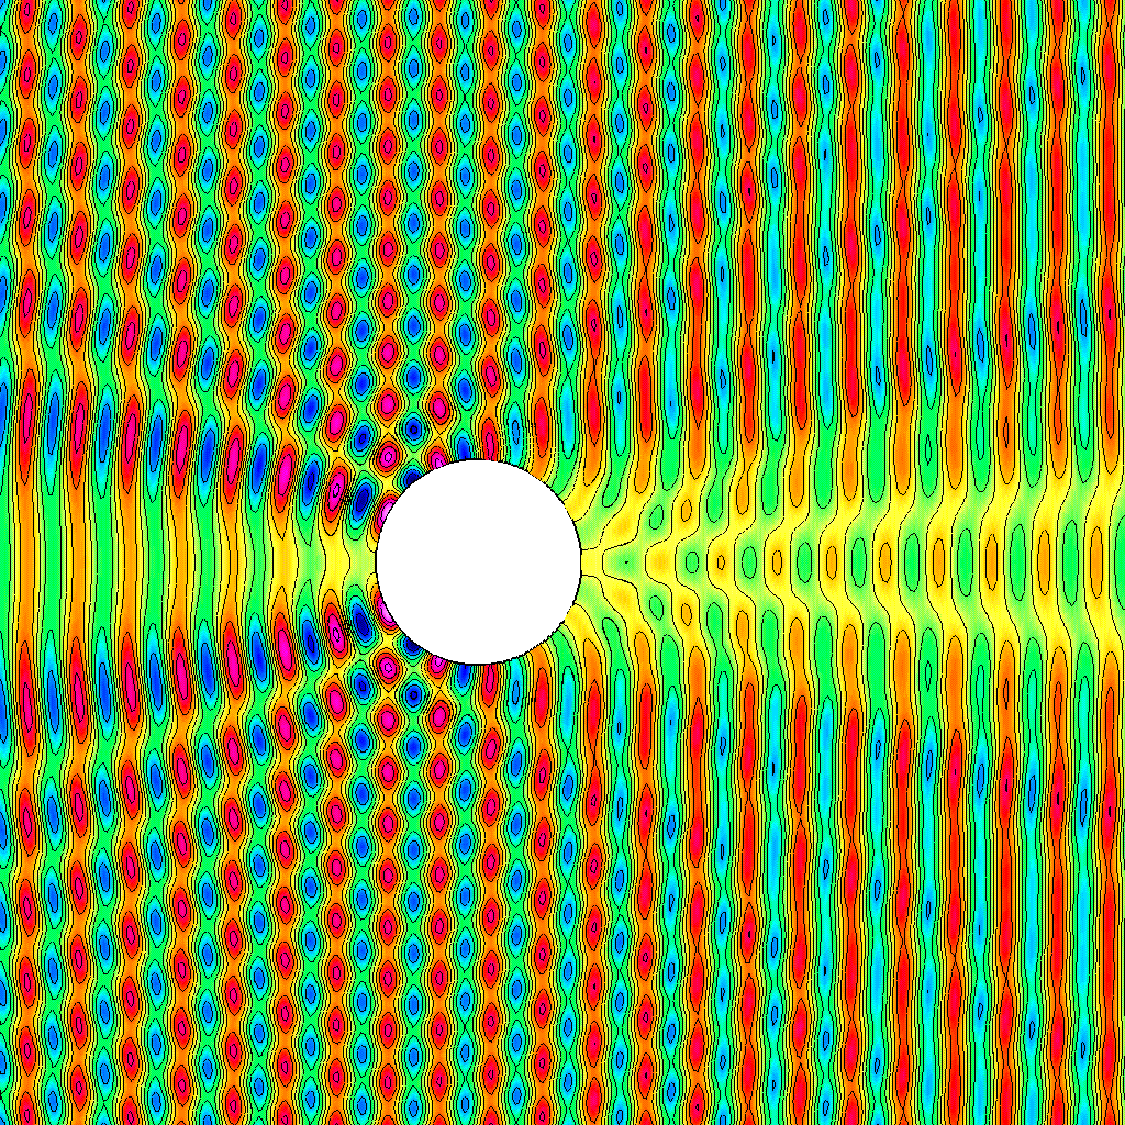
\includegraphics[width=\figWidth]{figures/scatCyl-cibc2-order4-k4-HzTotal}
%- \epsfig{file=\maxDoc/scatCyl.cibc2.order4.k4.ExTotal.ps,width=\figWidth}  
%-  \epsfig{file=\maxDoc/scatCyl.cibc2.order4.k4.EyTotal.ps,width=\figWidth}  
%-  \epsfig{file=\maxDoc/scatCyl.cibc2.order4.k4.HzTotal.ps,width=\figWidth}  
% \epsfig{file=\maxDoc/scatCyl.cibc2a.order4.k5.ExTotal.ps,width=\figWidth}  
% \epsfig{file=\maxDoc/scatCyl.cibc2a.order4.k5.EyTotal.ps,width=\figWidth}  
% \epsfig{file=\maxDoc/scatCyl.cibc2a.order4.k5.HzTotal.ps,width=\figWidth}  
\end{center}
\caption{Scattering of a plane wave by a cylinder. Total field $E_x$, $E_y$ and $H_z$ for $k a = 2$.}
\end{figure}



\subsection{Scattering by a sphere}

The scattering of a plane wave by a sphere is considered.

For an incident wave
\[
   \Ev^i = \hat{x} e^{-ikz}
\]
the total field is given by the series expansion
\begin{align*}
   E_r &= {i\cos(\phi)\over (kr)^2} 
              \sum_{n=1}^\infty (-i)^n (2n+1)\big[ \psi_n(kr) - b_n \zeta_n^{(1)}(kr)\big] P_n^1(\cos(\theta)) \\
   E_\theta &= {\cos(\phi)\over kr}
              \sum_{n=1}^\infty (-i)^n {2n+1 \over n(n+1)}
                 \big[ A_n {P_n^1(\cos(\theta)) \over \sin(\theta)}
                      +i B_n \partial_\theta P_n^1(\cos(\theta)) \big] \\
   E_\phi &= -{\sin(\phi)\over kr}
              \sum_{n=1}^\infty (-i)^n {2n+1 \over n(n+1)}
                 \big[ A_n \partial_\theta P_n^1(\cos(\theta))
                      +i B_n {P_n^1(\cos(\theta)) \over \sin(\theta)} \big] \\ 
\end{align*}
where
\begin{align*}
 A_n &= \psi_n(kr) - a_n \zeta_n^{(1)}(kr) \\
 B_n &= \psi_n'(kr) - b_n \zeta_n^{(1)'}(kr) \\
  j_n(z) &= \sqrt{\pi\over 2 z} J_{n+1/2}(z), ~~ h_n^{(1)}(z)= \sqrt{\pi\over 2 z} H_{n+1/2}(z) \\
  \psi(z) &= z j_n(z), ~~ \zeta_n^{(1)}(z)= z h_n^{(1)}(z), ~~ a_n={\psi_n(ka)\over \zeta_n^{(1)}(ka)}, ~~
       b_n ={\psi_n'(ka)\over \zeta_n^{(1)'}(ka)}
\end{align*}

The solution is computed on a large domain... 


% sib1b.order4
% -->t=4.0000e+00 dt=1.2e-02 Errors:[1.1268e-02,8.8984e-03,7.3602e-03,], max(u):[1.47e+00,1.32e+00,7.99e-01,]
% >>> Maxwell NFDTD: t=4.00e+00, dt=1.2e-02 TS=ME orderX=4 orderT=4 ad=0.10(order=4) |div(E)|=3.67e-02, (340 steps)
% -->t=5.0000e+00 dt=1.2e-02 Errors:[1.2654e-02,8.3613e-03,7.1347e-03,], max(u):[1.47e+00,1.32e+00,7.99e-01,]
% >>> Maxwell NFDTD: t=5.00e+00, dt=1.2e-02 TS=ME orderX=4 orderT=4 ad=0.10(order=4) |div(E)|=3.67e-02, (425 steps)
% -->t=6.0000e+00 dt=1.2e-02 Errors:[1.3470e-02,8.3779e-03,6.8293e-03,], max(u):[1.47e+00,1.32e+00,8.00e-01,]
% >>> Maxwell NFDTD: t=6.00e+00, dt=1.2e-02 TS=ME orderX=4 orderT=4 ad=0.10(order=4) |div(E)|=3.66e-02, (510 steps)

% **** sib2a.order4: bigger box [-4,4]^3
% -->t=4.0000e+00 dt=6.5e-03 Errors:[2.6988e-03,3.6437e-03,1.2048e-03,], max(u):[1.49e+00,1.33e+00,8.12e-01,]
% >>> Maxwell NFDTD: t=4.00e+00, dt=6.5e-03 TS=ME orderX=4 orderT=4 ad=0.10(order=4) |div(E)|=7.69e-03, (620 steps)
% -->t=5.0000e+00 dt=6.5e-03 Errors:[7.0185e-04,1.1130e-03,1.0399e-03,], max(u):[1.49e+00,1.33e+00,8.12e-01,]
% >>> Maxwell NFDTD: t=5.00e+00, dt=6.5e-03 TS=ME orderX=4 orderT=4 ad=0.10(order=4) |div(E)|=7.68e-03, (775 steps)
% -->t=6.0000e+00 dt=6.5e-03 Errors:[2.2152e-03,1.2944e-03,6.1221e-04,], max(u):[1.49e+00,1.33e+00,8.12e-01,]
% >>> Maxwell NFDTD: t=6.00e+00, dt=6.5e-03 TS=ME orderX=4 orderT=4 ad=0.10(order=4) |div(E)|=1.69e-02, (930 steps)
% -->t=7.0000e+00 dt=6.5e-03 Errors:[1.2599e-03,1.3647e-03,6.8481e-04,], max(u):[1.49e+00,1.33e+00,8.12e-01,]


% *****sib1x4.order4  161^3 (twice as fine again) 6M pts  top=1.3G
% -->t=3.0000e+00 dt=2.9e-03 Errors:[5.3265e-05,3.6572e-05,2.6581e-05,], max(u):[1.49e+00,1.33e+00,8.18e-01,]
% >>> Maxwell NFDTD: t=3.00e+00, dt=2.9e-03 TS=ME orderX=4 orderT=4 ad=0.10(order=4) |div(E)|=4.71e-04, |div(E)|/|grad(E)|=4.14e-06 (1020 steps)
% *****sib1x2.order4  81^3 (twice as fine) 907,000 pts
% -->t=3.0000e+00 dt=5.9e-03 Errors:[7.9950e-04,5.5375e-04,4.0260e-04,], max(u):[1.49e+00,1.33e+00,8.12e-01,]
% >>> Maxwell NFDTD: t=3.00e+00, dt=5.9e-03 TS=ME orderX=4 orderT=4 ad=0.10(order=4) |div(E)|=3.99e-03, |div(E)|/|grad(E)|=7.01e-05 (510 steps)
% *****sib1.order4  142,000 pts
% -->t=3.0000e+00 dt=1.2e-02 Errors:[1.1067e-02,7.8379e-03,5.6020e-03,], max(u):[1.47e+00,1.32e+00,8.01e-01,]
% >>> Maxwell NFDTD: t=3.00e+00, dt=1.2e-02 TS=ME orderX=4 orderT=4 ad=0.10(order=4) |div(E)|=3.71e-02, |div(E)|/|grad(E)|=1.25e-03 (255 steps)

\begin{table}[hbt]
\begin{center}
\begin{tabular}{|l|c|c|c|c|c|} \hline\hline 
grid           & $h_0/h$ &    $E_x$       &  $E_y$       & $E_z$        & $\grad\cdot\uv$\\ \hline 
sib1.order4    &   1     &  $1.11e-2$  & $7.84e-3$ & $5.60e-3$ & $3.71e-2$   \\ \hline
sib1x2.order4  &   2     &  $8.00e-4$  & $5.54e-4$ & $4.03e-4$ & $3.99e-3$   \\ \hline
sib1x4.order4  &   4     &  $5.33e-5$  & $3.66e-5$ & $2.66e-5$ & $4.71e-4$   \\ \hline
   rate        &         &  $       $  & $       $ & $       $ & $       $   \\ \hline
\end{tabular}
\caption{Errors in the scattering of a plane wave by a sphere, order=$4$, $t=3$. Initial conditions and
   far field boundary conditions set to the exact solution}\label{table:scatSphere}
\end{center}
\end{table}

\begin{table}[hbt]
\begin{center}
\begin{tabular}{|l|c|c|c|c|c|} \hline\hline 
grid  & N &  $E_x$ &  $E_y$ & $E_z$ & $\grad\cdot\uv$\\ \hline 
         sib1.order4 &    40 &$1.3 e-2$ &$8.1 e-3$ &$6.7 e-3$ &$3.9 e-3$  \\ \hline
       sib1x2.order4 &    80 &$9.3 e-4$ &$5.8 e-4$ &$4.8 e-4$ &$4.2 e-4$  \\ \hline
       sib1x4.order4 &   160 &$6.2 e-5$ &$3.9 e-5$ &$3.2 e-5$ &$5.4 e-5$  \\ \hline
    rate            &     &       $3.86$ &       $3.86$ &       $3.85$ &       $3.09$  \\ \hline\hline
\end{tabular}
\caption{Errors in the scattering of a plane wave by a sphere, order=$4$, $t=2.$, sib, scattering, cfl=.95,
   Initial conditions and far field boundary conditions set to the exact solution}\label{table:mx.sib}
\end{center}
\end{table}

% ----------------------------------------------------------------------------------
\clearpage
\subsection{Computing eigenvalues of an L-shaped domain with time series}

\renewcommand{\figWidth}{.5\linewidth}
\begin{figure}
\begin{center}
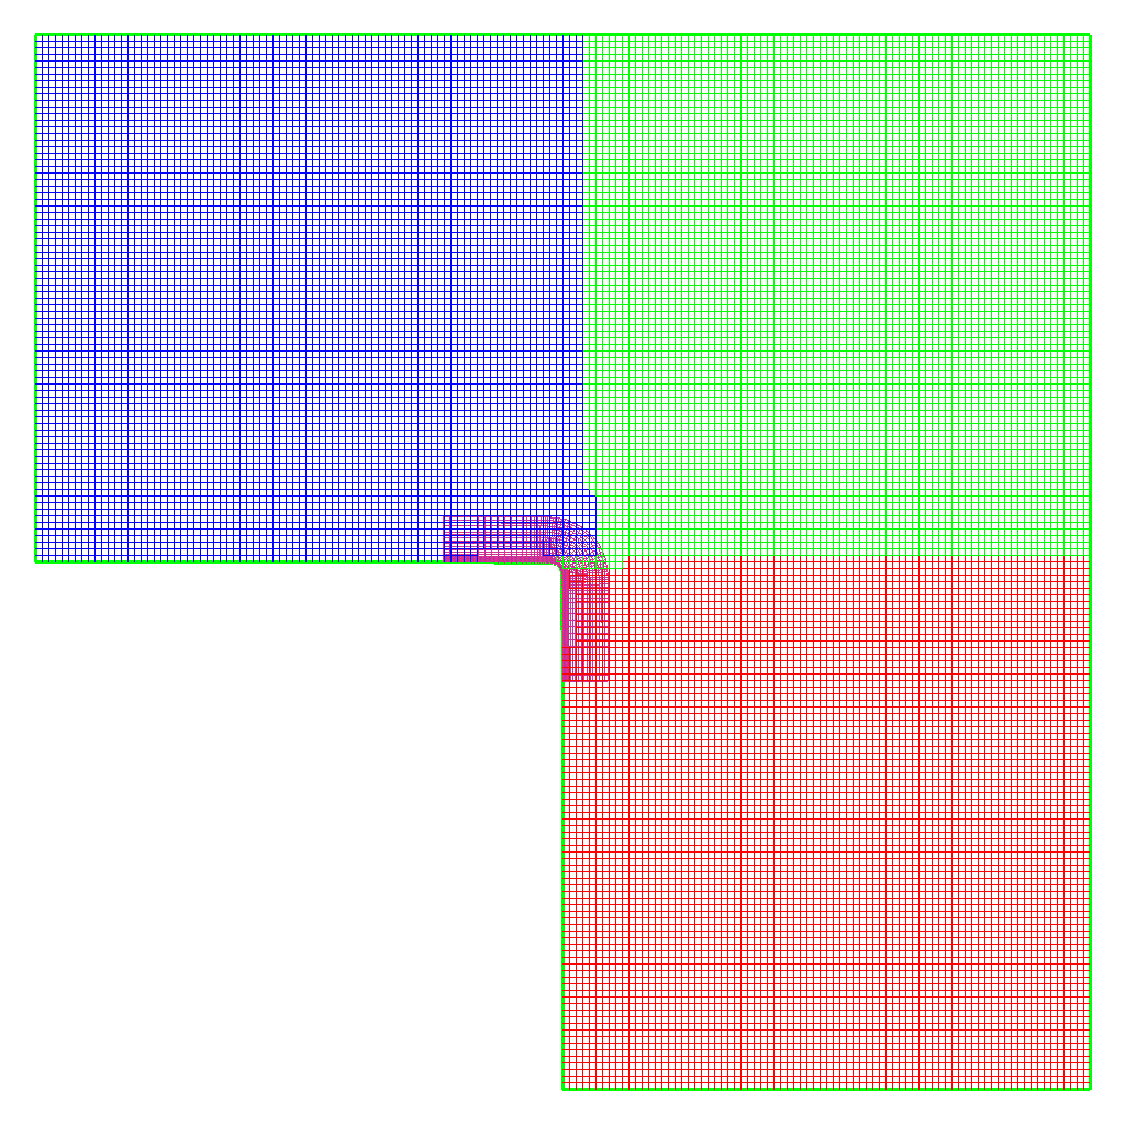
\includegraphics[width=\figWidth]{figures/lgrid2e-order4-grid}
% \epsfig{file=\maxDoc/lgrid2e.order4.grid.ps,width=\figWidth}
\end{center}
\caption{Grid for the L-shaped region.}
\end{figure}
\renewcommand{\figWidth}{.495\linewidth}
\begin{figure}
\begin{center}
\includegraphics[width=\figWidth]{figures/psd-lgrid2e-4}
\includegraphics[width=\figWidth]{figures/eigenValues-relErr-lgrid2e-4}
% \epsfig{file=\maxDoc/psd-lgrid2e-4.eps,width=\figWidth}  
% \epsfig{file=\maxDoc/eigenValues-relErr-lgrid2e-4.eps,width=\figWidth}  
\end{center}
\caption{Left: Power-Spectral-Density for the L-shaped region, lgrid2e.order4. 
         Right: relative errors in the eigenvalues.}
\end{figure}

% ----------------------------------------------------------------------------------
\clearpage
\subsection{Computing eigenvalues of a cylinder with time series}

\renewcommand{\figWidth}{.495\linewidth}
\begin{figure}
\begin{center}
\includegraphics[width=\figWidth]{figures/psd-tube3-4-Ez}
\includegraphics[width=\figWidth]{figures/eigenValues-relErr-tube3-4-Ez}
% \epsfig{file=\maxDoc/psd-tube3-4-Ez.eps,width=\figWidth}  
% \epsfig{file=\maxDoc/eigenValues-relErr-tube3-4-Ez.eps,width=\figWidth}  
\end{center}
\caption{Left: Power-Spectral-Density for a cylinder.
         Right: relative errors in the eigenvalues.}
\end{figure}

% ====================================================================================================
\clearpage
\subsection{Computing eigenvalues of a pill-box with time series}

\renewcommand{\figWidth}{.495\linewidth}
\begin{figure}
\begin{center}
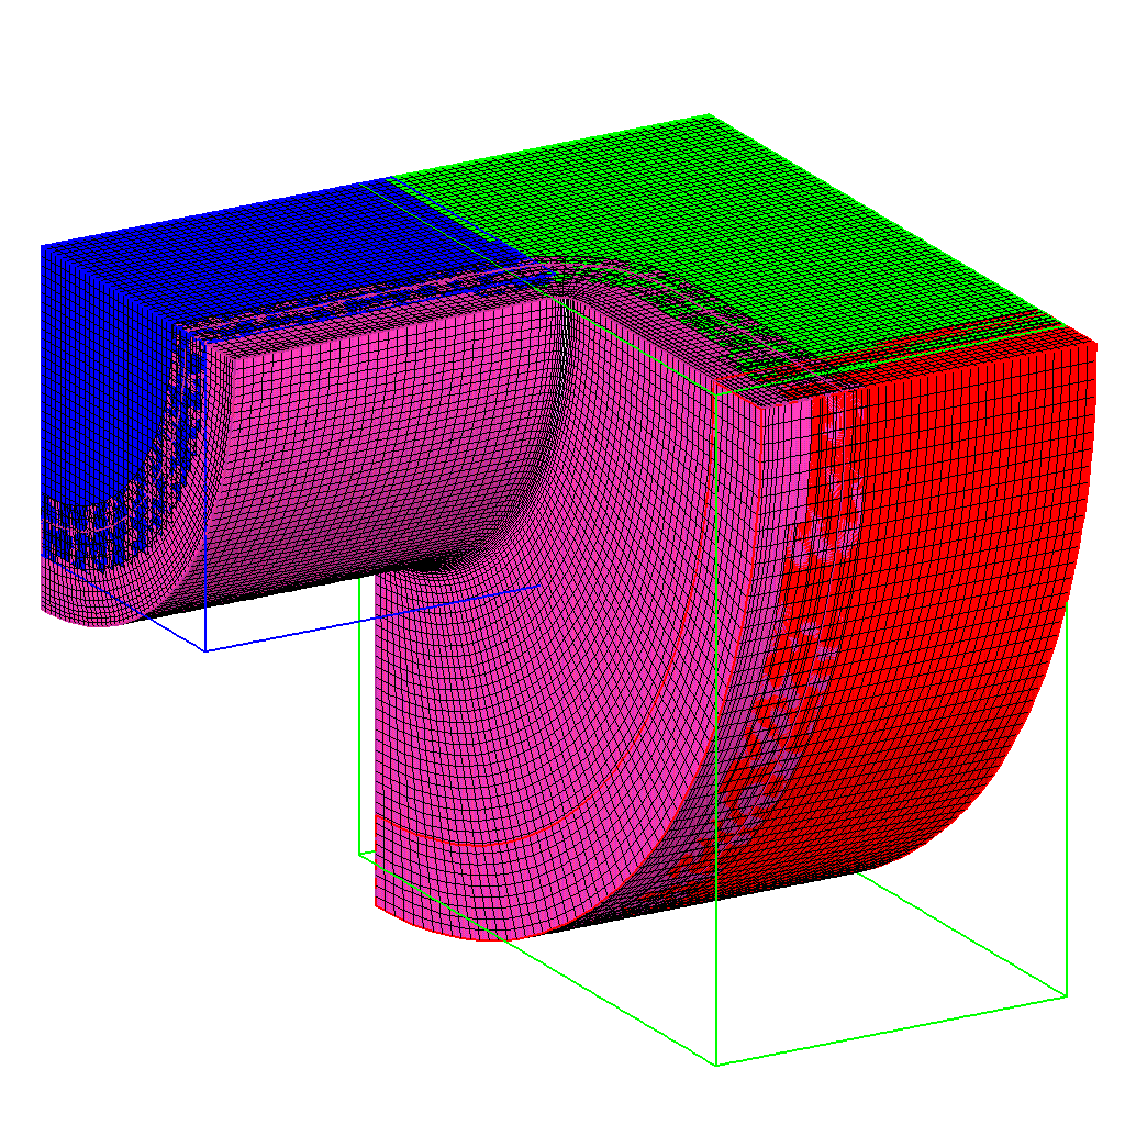
\includegraphics[width=\figWidth]{figures/pillBox2-order4-grid}
% \epsfig{file=\maxDir/pillBox2.order4-grid.ps,width=\figWidth}  
\end{center}
\caption{Grid for a pill-box.}
\end{figure}


% ====================================================================================================
\clearpage
\subsection{Computing eigenvalues of a sphere with time series}

The first set of eigenvalues for modes inside a sphere are given by the the positive roots of 
\begin{align*}
  J_{n+\half}(\sqrt{\lambda_{np}}~ a)=0 , \qquad n=1,2,3,\ldots \qquad p=1,2,3,\ldots
\end{align*}
A few values are $\sqrt{\lambda_{11}}~ a \approx 4.49$, $\sqrt{\lambda_{2,1}}~ a \approx 5.76$,
$\sqrt{\lambda_{3,1}}~ a \approx 6.99$ 
$\sqrt{\lambda_{1,2}}~ a \approx 7.73$ 


The second set of eigenvalues are given by the the positive roots of 
\begin{align*}
  J_{n+1+\half}(z_{np})
     + {n+1\over z_{np}}J_{n+\half}(z_{np})=0 , 
                \qquad n=1,2,3,\ldots \qquad p=1,2,3,\ldots
\end{align*}
for $z_{np}=\sqrt{\lambda_{np}}~ a$. 
A few values are $\sqrt{\lambda_{11}}~ a \approx 2.743$, $\sqrt{\lambda_{2,1}}~ a \approx 3.87$,
$\sqrt{\lambda_{1,2}}~ a \approx 6.11$ and $\sqrt{\lambda_{2,2}}~ a \approx 7.44$

Table~(\ref{tab:eigSphere}) shows the PSD for a sphere and the relative errors in 
some of the eigenvalues.

\renewcommand{\figWidth}{.475\linewidth}
\begin{figure}
\begin{center}
\includegraphics[width=\figWidth]{figures/psd-bis2e-4-T200}
\includegraphics[width=\figWidth]{figures/eigenValues-relErr-bis2e-4-T200}
% \epsfig{file=\maxDoc/psd-bis2e-4-T200.eps,width=\figWidth}  
% \epsfig{file=\maxDoc/eigenValues-relErr-bis2e-4-T200.eps,width=\figWidth}  
\end{center}
\caption{Left: Power-Spectral-Density for a sphere, bis2e.order4. Right: relative errors in the eigenvalues.}
\label{tab:eigSphere}
\end{figure}


% ===================================================================================================
\clearpage
\subsection{Scattering of a plane wave by a dielectric cylinder}

Table~\ref{table:mx.innerOuter} shows convergence results for the scattering of a plane
wave by a dielectric cylinder with different material properties.

\begin{table}[hbt]
\begin{center}
\begin{tabular}{|l|c|c|c|c|c|} \hline\hline 
grid  & N &  $E_x$ &  $E_y$ & $H_z$ & $\|\grad\cdot\Ev\|/\|\grad\Ev\|$\\ \hline 
innerOuter2.order4.hdf &     1 &$6.0 e-3$ &$1.2 e-2$ &$1.4 e-2$ &$4.1 e-3$  \\ \hline
innerOuter4.order4.hdf &     2 &$4.0 e-4$ &$7.9 e-4$ &$8.9 e-4$ &$2.7 e-4$  \\ \hline
innerOuter8.order4.hdf &     4 &$2.6 e-5$ &$5.0 e-5$ &$5.6 e-5$ &$1.8 e-5$  \\ \hline
    rate            &     &       $3.93$ &       $3.97$ &       $3.97$ &       $3.93$  \\ \hline\hline
\end{tabular}
\caption{nfdtd, order=$4$, $t=1.$, innerOuter, material interface, $k_x=2$, inner $\epsilon=1/4$,
   outer $\epsilon=1$, cfl=.8, ad=.5}\label{table:mx.innerOuter}
\end{center}
\end{table}


% ====================================================================================================
\clearpage
\subsection{Serial performance and memory usage}


% ------------ Table for LaTeX -------------------------------
\begin{table}[hbt]
\begin{center}\footnotesize
\begin{tabular}{|l|r|r|r|r|} \hline
  Timings:   &  seconds &    sec/step  &  sec/step/pt &  \%    \\ \hline
total~time\dotfill &   1.85e+03 &   1.73e+00 &   4.55e-07 & 100.000 \\ 
setup~and~initialize\dotfill &   1.34e+00 &   1.25e-03 &   3.29e-10 &   0.072 \\ 
initial~conditions\dotfill &   5.57e+01 &   5.20e-02 &   1.37e-08 &   3.004 \\ 
advance\dotfill &   1.79e+03 &   1.67e+00 &   4.39e-07 &  96.502 \\ 
~~advance~rectangular~grids\dotfill &   1.32e+03 &   1.24e+00 &   3.25e-07 &  71.420 \\ 
~~advance~curvilinear~grids\dotfill &   2.59e+02 &   2.42e-01 &   6.35e-08 &  13.950 \\ 
~~~(advOpt)\dotfill &   1.37e+03 &   1.28e+00 &   3.36e-07 &  73.894 \\ 
~~add~dissipation\dotfill &   3.09e+01 &   2.89e-02 &   7.59e-09 &   1.668 \\ 
~~boundary~conditions\dotfill &   1.97e+02 &   1.84e-01 &   4.84e-08 &  10.632 \\ 
~~interpolation\dotfill &   8.51e+00 &   7.94e-03 &   2.09e-09 &   0.459 \\ 
get~errors\dotfill &   6.34e+00 &   5.92e-03 &   1.56e-09 &   0.342 \\ 
compute~dt\dotfill &   9.65e-03 &   9.01e-06 &   2.37e-12 &   0.001 \\ 
plotting\dotfill &   2.82e+00 &   2.63e-03 &   6.91e-10 &   0.152 \\ 
 \hline 
\end{tabular}
\end{center}
\caption{grid=cic5.order4.hdf, 3805020 grid points, 9400 interp points, 1071 steps taken, 1 processors.}
\label{tab:cic5.order4.hdf}
\end{table}

%  ------------------------------------------------------------------------------ 
%    Memory usage                   Mbytes    real/point  real/component  percent   
%  size of: cgfields=   261.27, fields=     0.00, fn=     6.69, cgdiss=     0.00, err=    87.09 (MB)
%  CompositeGrid..................    76.72       2.64         0.88        17.7%  
%  finite difference operators....     0.01       0.00         0.00         0.0%  
%  Interpolant....................     0.16       0.01         0.00         0.0%  
%  Grid functions.................   355.05      12.23         4.08        81.8%  
%  local arrays...................     2.23       0.08         0.03         0.5%  
%  total (of above items).........   434.17      14.96         4.99       100.0%  
%  ------------------------------------------------------------------------------ 


% ------------ Table for LaTeX -------------------------------
\begin{table}[hbt]
\begin{center}\footnotesize
\begin{tabular}{|l|r|r|r|r|} \hline
  Timings:   &  seconds &    sec/step  &  sec/step/pt &  \%    \\ \hline
total~time\dotfill &   3.65e+02 &   4.80e+00 &   1.94e-06 & 100.000 \\ 
setup~and~initialize\dotfill &   9.06e+00 &   1.19e-01 &   4.83e-08 &   2.484 \\ 
initial~conditions\dotfill &   9.09e+00 &   1.20e-01 &   4.84e-08 &   2.492 \\ 
advance\dotfill &   3.53e+02 &   4.65e+00 &   1.88e-06 &  96.899 \\ 
~~advance~rectangular~grids\dotfill &   6.86e+01 &   9.03e-01 &   3.66e-07 &  18.821 \\ 
~~advance~curvilinear~grids\dotfill &   2.05e+02 &   2.70e+00 &   1.09e-06 &  56.236 \\ 
% ~~advOpt~~~~\dotfill &   8.05e+01 &   1.06e+00 &   4.29e-07 &  22.066 \\ 
~~boundary~conditions\dotfill &   3.96e+01 &   5.21e-01 &   2.11e-07 &  10.864 \\ 
~~interpolation\dotfill &   3.69e+01 &   4.86e-01 &   1.97e-07 &  10.128 \\ 
compute~dt\dotfill &   5.80e-02 &   7.63e-04 &   3.09e-10 &   0.016 \\ 
plotting\dotfill &   2.22e+00 &   2.92e-02 &   1.18e-08 &   0.608 \\ 
 \hline 
\end{tabular}
\end{center}
\caption{grid=bis3e.order4.hdf, 2468750 grid points, 236176 interp points, 76 steps taken, 1 processors.}
\label{tab:bis3e.order4.hdf}
\end{table}


\begin{table}[hbt]
\begin{center}\footnotesize
\begin{tabular}{|l|r|r|r|r|} \hline
%  ------------------------------------------------------------------------------ 
   Memory usage       &            Mbytes  &   real/point &  real/var  &  percent   \\ \hline\hline
 CompositeGrid                     &  71.70 &      3.81 &        1.27  &      31.9  \\
 finite difference operators       &   0.01 &      0.00 &        0.00  &       0.0  \\
 Interpolant                       &   5.42 &      0.29 &        0.10  &       2.4  \\
 Grid functions                    & 147.34 &      7.82 &        2.61  &      65.6  \\ \hline
 total (of above items)            & 224.48 &     11.92 &        3.97  &     100.0  \\ \hline
%  ------------------------------------------------------------------------------ 
\end{tabular}
\end{center}
\caption{Sphere, bis3e.order4.hdf, 2468750 grid points, 236176 interp points, 1 processors.
         Memory usage. (Memory from top=231M) }
\label{tab:mem:bis3e.order4}
\end{table}


% -----------------------------------------------------------------------------------
\clearpage
\subsection{Parallel performance}

Here are some results from running the code in parallel.

\begin{table}[hbt]
\begin{center}\footnotesize
\begin{tabular}{|c|c|c|} \hline 
     NP       & sec/step   & ratio      \\   \hline\hline 
     1        &  $2.14$    & $ 1. $     \\ 
     2        &  $1.01$    & $ 2.1$     \\ 
     3        &  $.59 $    & $ 3.6$     \\ \hline 
\end{tabular}	
\qquad
\begin{tabular}{|c|c|c|} \hline 
     NP       & sec/step   & ratio \\   \hline\hline 
     1        &  $.   $    & $ 1. $   \\ 
     2        &  $5.10$    & $    $   \\ 
     3        &  $2.69$    & $    $   \\ \hline 
\end{tabular}		
\qquad

\end{center}		
\caption{Square. Left: square2048.order4, 4.2M grid points.
                 Right: square4096.order4, 16.8M grid points. Dell workstations 2.2GHz pentium.}
 \label{tab:box} 
\end{table}

\begin{table}[hbt]
\begin{center}\footnotesize
\begin{tabular}{|c|c|c|} \hline 
     NP       & sec/step   & ratio \\   \hline\hline 
     1        &  $11.8$    & $ 1. $   \\ 
     2        &  $5.67$    & $    $   \\ 
     4        &  $3.00$    & $    $   \\ \hline 
\end{tabular}		
\qquad
\begin{tabular}{|c|c|c|} \hline 
     NP       & sec/step   & ratio \\   \hline\hline 
     1        &  $61.3$    & $ 1. $   \\ 
     2        &  $29.0$    & $    $   \\ 
     4        &  $14.2$    & $    $   \\ \hline 
\end{tabular}
\end{center}		
\caption{Cylinder. Left tube4.order4, 2.6e6 grid points. Right: tube5.order4, 17.3e6 grid points. 
Compaq gps320, 1 GHz alpha Processor.}
 \label{tab:box} 
\end{table}

% \begin{table}[hbt]
% \begin{center}\footnotesize
% \begin{tabular}{|c|c|c|} \hline 
%      NP       & sec/step   & ratio \\   \hline\hline 
%      1        &  $61.3$    & $ 1. $   \\ 
%      2        &  $29.0$    & $    $   \\ 
%      4        &  $14.2$    & $    $   \\ \hline 
% \end{tabular}		
% \end{center}		
% \caption{Cylinder,tube5.order4, 17.3e6 grid points, Compaq gps320, 1 GHz alpha Processor.}
%  \label{tab:box} 
% \end{table}
